%\graphicspath{{~/Pictures/Screenshots/}}
\graphicspath{{~/Documents/MobAppDev/SecondTask/PNG}}
\section*{\LARGE{Цель практической работы}}
\addcontentsline{toc}{section}{Цель практической работы}
В практической работе была рассмотренно как использовать базовые возможности
платформы для управления ресурсами для оптимизации приложения
под различные Android-совместимые устройства, и разместить его в
единственном APK-файле.

\newpage

\section*{\LARGE{Выполнение практической работы}}
\addcontentsline{toc}{section}{Выполнение практической работы}

\section{Поддержка различных языков}
Размещение строковых констант в отдельном файле считается хорошим
тоном. В каждом проекте Andoid для строковых констант существует
специальная директория.\par
Когда создются проекты используя инструменты Android SDK, то
директория \texttt{res/} создается автоматически в корневой директории
проекта. Также для каждого из типов ресурсов создаются собственные
поддиректории, а так же несколько стандартных файлов. Например
файл \texttt{res/values/strings.xml}, в котором хранятся строковые константы.

\subsection{Создание директорий для поддержки различных языков}
Для поддержки нескольких языков, необходимо создать в директории res
несколько дополнительных директорий values, содержащих в имени ISO
коды языков. К примеру, директория values-ru будет включать в себя ресурсы
для поддержки русского языка.
Android загружает нужные ресурсы в соответствии с настройками
локализации устройства, на котором было запущено приложение.
Чтобы включить поддержку нескольких языков, создали
необходимые поддиректории и файлы строковых ресурсов. К примеру, как
на рисунке \ref{fig:res:values}.

\begin{figure}[h!tp]
	\centering
	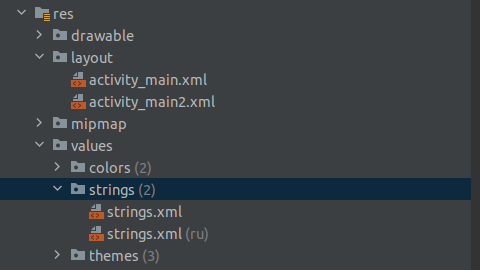
\includegraphics[width=0.8\textwidth]{Screenshot from 2023-02-20 18-03-12.png}
	\caption{Директория ресурсов проекта}
	\label{fig:res:values}
\end{figure}

Добавили строковые константы в каждый из файлов.\par
При запуске Android самостоятельно выберет подходящий файл в
соответствии с настройками локализации устройства.\par
Пример содержания файлов строковых ресурсов для различных
языков:
\begin{itemize}
	\item Английский (по умолчанию), /values/strings.xml,
		рисунок~\ref{fig:res:values:en}.
		\begin{figure}[h!tp]
			\centering
			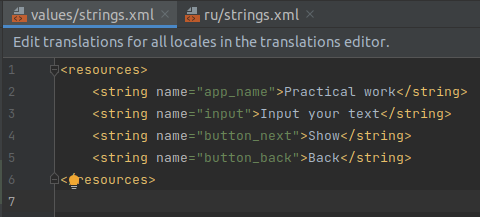
\includegraphics[width=0.7\textwidth]{Screenshot from 2023-02-20 18-13-18.png}
			\caption{Файл английских ресурсов}
			\label{fig:res:values:en}
		\end{figure}
	\item Русский, /values-ru/strings.xml,
		рисунок~\ref{fig:res:values:ru}.
		\begin{figure}[h!tp]
			\centering
			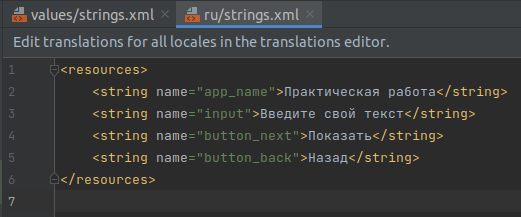
\includegraphics[width=0.7\textwidth]{Screenshot from 2023-02-20 18-13-33.png}
			\caption{Файл русских ресурсов}
			\label{fig:res:values:ru}
		\end{figure}
\end{itemize}

\subsection{Использование строковых ресурсов}
Можно ссылаться на строковые ресурсы из программного кода и других
XML файлов, используя название ресурса, которое задается в свойстве name
элемента \texttt{<string>}.\par
На строковый ресурс можно ссылаться из XML файлов разметки,
используя синтаксис \texttt{@string/<string\_name>}, всякий раз,
когда требуется строковое значение для свойства, как показано
на рисунке~\ref{fig:xml:string}.
\begin{figure}[h!tp]
	\centering
	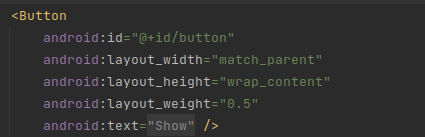
\includegraphics[width=0.8\textwidth]{Screenshot from 2023-02-20 18-33-17.png}
	\caption{Использование ресурсов в xml файле}
	\label{fig:xml:string}
\end{figure}

\section{Поддержка устройств с различными экранами}
Экраны Android устройств различаются по двум основным параметрам:
размер и разрешение. Это значит, что приложение
может быть установлено на устройствах с различными размерами и
разрешениями экрана. Чтобы оптимизировать приложение под различные
размеры и разрешения, оно должно содержать разные ресурсы под каждый
вид экрана.

\begin{itemize}
	\item Существует четыре обобщенных размера: маленький (small),
		нормальный(normal), большой(large), очень большой(x-large).
	\item Также существует четыре вида разрешений: низкое (low), среднее
		(mdpi), высокое (hdpi), очень высокое (xhdpi).
\end{itemize}

Чтобы использовать разную разметку и изображения для разных экранов,
необходимо размещать данные ресурсы в различные директории, точно
также, как мы это делали со строками для различных языков.\par
Также следует помнить об ориентации экрана (альбомная (landscape) или
портретная (portrait)), она так же считается отдельным размером и для
многих приложений необходимо отдельно оптимизировать разметку для
двух ориентаций.

\subsection{Создание различной разметки}
Чтобы оптимизировать пользовательский интерфейс под различные размеры
экрана, необходимо создать собственные файлы разметки для каждого из
размеров, которые вы хотите поддерживать. Каждый файл разметки должен
быть сохранен в соответствующей директории, название которой
заканчивается строкой \texttt{<screen\_size>}. Например, файл разметки для
больших экранов должен быть сохранен в директории \texttt{res/layout-large/}.

Директория проекта, который включает в себя стандартную разметку и разметку
для больших экранов, показан на рисунку \ref{fig:res:layout}.
\begin{figure}[h!tp]
	\centering
	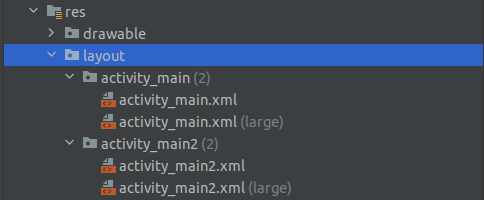
\includegraphics[width=0.8\textwidth]{Screenshot from 2023-02-20 19-31-44.png}
	\caption{Разметка для разный размеров экрана}
	\label{fig:res:layout}
\end{figure}

\section{Использование различных изображений}
Растровые изображения нужно создавать для каждого из основных
разрешений: низкого, среднего, высокого и очень высокого. Это позволит
добиться отличного качества и производительности на устройствах с любым
разрешением.\par
Чтобы создать такие изображения, создали базовый вариант в векторном
формате, а затем экспортировали его в растровый формат для каждого
разрешения, используя следующую шкалу размеров:

\begin{itemize}
	\item xhdpi: 2.0
	\item hdpi: 1.5
	\item mdpi: 1.0 (базовый размер)
	\item ldpi: 0.75
\end{itemize}

Это означает, что если создали картинку размером 200×200 пикселей для
xhdpi устройств, то для остальных устройств будут такие размеры: 150x150
для hdpi, 100×100 для mdpi и 75x75 для ldpi устройств.
После этого разместили файлы в соответствующих директориях, как показано
на рисунке~\ref{fig:res:drawable}.
\begin{figure}[h!tp]
	\centering
	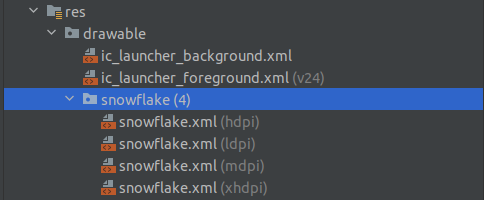
\includegraphics[width=0.8\textwidth]{Screenshot from 2023-02-20 20-10-08.png}
	\caption{Разметка для разный размеров экрана}
	\label{fig:res:drawable}
\end{figure}

\section{Поддержка различных версий Android}
В то время, как последние версии Andoid часто добавляют в API
великолепные возможности, вы должны продолжать поддерживать старые
версии Android до тех пор, пока большинство устройств не получат
обновление. В этом уроке мы рассмотрим как используя широкие
возможности последних API также продолжать поддержку старых версий
Android.\par
Диаграмма используемых версий регулярно обновляется и показывает
соотношение установленных версий Android. Диаграмма строится на основе
статистики из Google Play Store. В целом, хорошей практикой является
поддержка 90\% активных устройств при нацеливании на последние версии.

\subsection{Указание минимальной и целевой версии API}
В файле \texttt{AndroidManifest.xml} описывается какие версии Android
поддерживает приложение. Конкретно указываются атрибуты
\texttt{minSdkVersion} и \texttt{targetSdkVersion} для
элемента \texttt{<uses-sdk>}, которые указывают на минималную версию
с которым ваше приложение совместимо и максимальную версию,
на которой вы разрабатывали и тестировали приложение
(Рисунок~\ref{fig:manifest}).
\begin{figure}[h!tp]
	\centering
	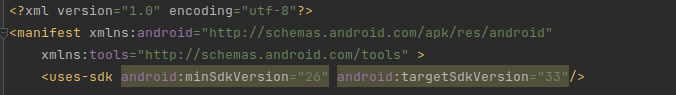
\includegraphics[width=0.8\textwidth]{Screenshot from 2023-02-20 20-20-10.png}
	\caption{Разметка для разный размеров экрана}
	\label{fig:manifest}
\end{figure}

\subsection{Получение версии Android во время выполнения приложения}
Android хранит специальный код для каждой из версий в виде константы в
классе Build.\par
В коде, изображенном на рисунке \ref{fig:code:vsdk} задает условие,
чтобы функции, доступные в более высоких версиях API выполнялись,
только если данный API доступен на устройстве.
\begin{figure}[h!tp]
	\centering
	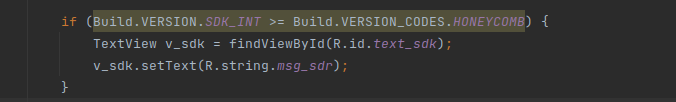
\includegraphics[width=0.8\textwidth]{Screenshot from 2023-02-20 20-37-17.png}
	\caption{Проверка версии SDK}
	\label{fig:code:vsdk}
\end{figure}

\section{Использование встроенных тем и стилей}
Android содержит стандартные темы интерфейса, которые позволяют
приложению выглядеть как одно целое с системой. Эти темы легко
использовать в приложении, указав их в файле манифеста. При
использовании встроенных тем, приложение будет «следить за модой» и
выглядеть по новому с каждым новым выпуском Android.\par
Пример, в котором явлению устанавливается ночная тема,
показан на рисунке~\ref{fig:manifest:theme}.
\begin{figure}[h!tp]
	\centering
	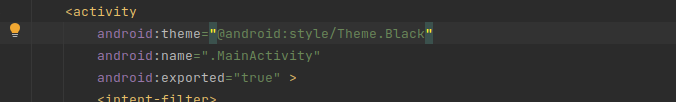
\includegraphics[width=0.8\textwidth]{Screenshot from 2023-02-20 21-00-16.png}
	\caption{Устанавливаем тему активити}
	\label{fig:manifest:theme}
\end{figure}

\section{Жизненный цикл явлений}
Когда пользователь просматривает приложение, выходит из него и снова
открывает, экземпляры Activity вашего приложения переключаются между
различными состояниями их жизненного цикла. К примеру, когда впервые
запускается приложение, оно занимает экран устройства и получает фокус
пользователя. В это время система вызывает некоторые методы управления
жизненным циклом явлений, отрисовывает интерфейс пользователя и другие
компонунты. Если открыли другое явление или другое приложение, система
выполняет другие методы управления жизненным циклом, теперь первое явление
уйдет в режим ожидания (в котором оно невидимо, но экземпляр класса
Activity и его состояние остаются неизменными).

\subsection{Запуск явлений}
В отличие от других парадигм программирования, в которых приложения
запускаются при помощи метода main(), Android использует функции
обратного вызова экземпляра Activity, соответствующие этапам его
жизненного цикла. Методы вызываются в различной последовательности при
запуске явления и при его завершении

\subsection{Функции обратного вызова жизненного цикла}
Во время существования явления, система вызывает методы один за другим,
подобно движению к вершине пирамиды. Каждая стадия жизненного цикла
соответствует отдельному шагу. Вершина пирамиды – это точка, в которой
явление видимо и пользователь может с ним взаимодействовать
(см.~рис.~\ref{fig:activity:ll}).\par
Когда пользователь покидает явление, система вызывает другие методы,
которые спускают явление к основанию пирамиды. В некоторых случаях
явление может спустить только на один шаг и перейти в режим ожидания
(например если пользователь переключился на другое приложение), а затем
вернуться обратно в вершину (если пользователь заново открыл явление) и
начать выполнение с места прерывания.
\begin{figure}[h!tp]
	\centering
	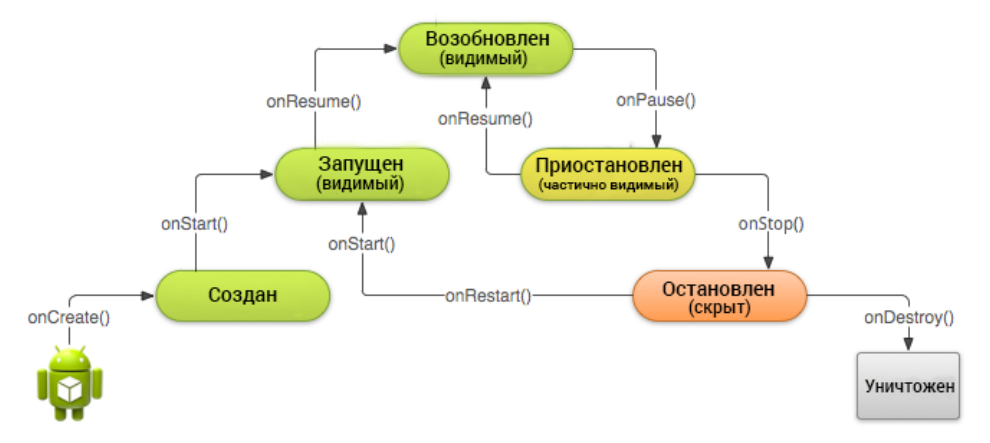
\includegraphics[width=0.8\textwidth]{Screenshot from 2023-02-21 10-58-53.png}
	\caption{Жизненный цикл Activity}
	\label{fig:activity:ll}
\end{figure}

Так при запуске Activity первым запускается метод \texttt{onCreate()}.
Начало этого метода в java коде показана
на рисунке~\ref{fig:activity:onCreate}.
\begin{figure}[h!tp]
	\centering
	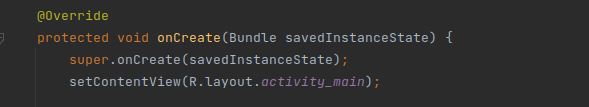
\includegraphics[width=0.8\textwidth]{Screenshot from 2023-02-21 11-02-22.png}
	\caption{Жизненный цикл Activity}
	\label{fig:activity:onCreate}
\end{figure}

\subsection{Объявление главного явления}
Когда пользователь щелкает по иконке приложения, система
вызывает метод onCreate() явления, который объявлен главным. Это
явление, которое является точкой входа в пользовательский интерфейс
приложения.\par
В файле манифеста \texttt{AndroidManifest.xml}, который находится в корневой
директории проекта, можно указать какое из явлений будет главным.
Главное явление должно содержать раздел \texttt{<intent-filter>},
включающий действие \texttt{MAIN} и категорию \texttt{LAUNCHER}
(Рисунок~\ref{fig:manifest:MAIN}).
\begin{figure}[h!tp]
	\centering
	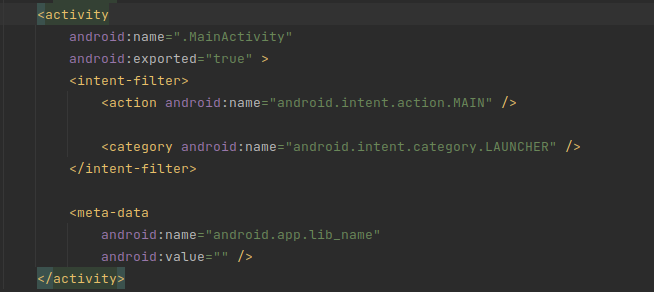
\includegraphics[width=0.8\textwidth]{Screenshot from 2023-02-21 11-20-40.png}
	\caption{Файл манифеста с объявлением главного явления}
	\label{fig:manifest:MAIN}
\end{figure}

\subsection{Создание экземпляра явления}
Часто приложения состоят из нескольких явлений, для выполнения
различных действий. Система всегда создает экземпляр любого явления,
вызывая метод onCreate().\par
В методе onCreate() описываются начальные действия явления, которые
выполняются однократно во время всего жизненного цикла, к примеру
создание пользовательского интерфейса и инициализация переменных
класса.\par
На рисунке~\ref{fig:activity:onCreate:content} приведен пример
реализации метода onCreate(), в котором подключается и настраивается XML
разметка интерфейса пользователя и определяются некоторые переменные.
\begin{figure}[h!tp]
	\centering
	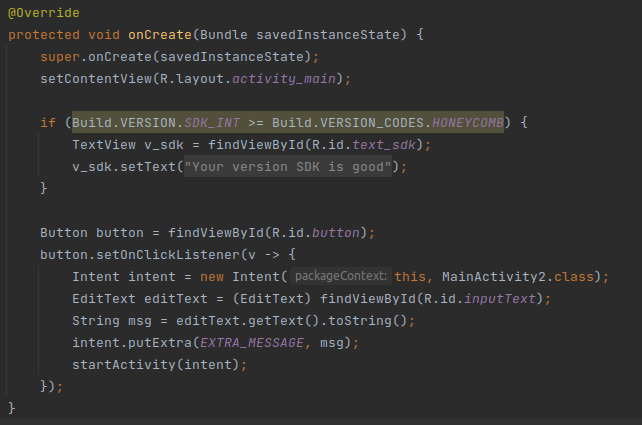
\includegraphics[width=0.8\textwidth]{Screenshot from 2023-02-21 11-24-19.png}
	\caption{Содержание метода onCreate}
	\label{fig:activity:onCreate:content}
\end{figure}
После выполнения onCreate() система вызывает методы onStart() и
onResume(). Важно помнить, что явление никогда не задерживается в состоянии
\textbf{Создано} или \textbf{Запущено}. Технически явление становится
видимым уже при вызове onStart(), однако состояние быстро меняется на
Возобновлено и явление будет находиться в этом состоянии до тех пор,
пока какое-либо событие (например телефонный вызов или отключение экрана
устройства) не заставит его измениться.

\subsection{Приостановка и возобновление явлений}
Во время использования приложения, явление может перекрываться другими
визуальными компонентами, из-за чего происходит его \textbf{приостановка}. К
примеру, при открытии диалога явление приостанавливается. Явление может
оставаться частично видимым, однако будет оставаться приостановленным
до тех пор, пока не получит фокус. Если же явление скрыто полностью
и невидимо, оно переходит в состояние \textbf{остановлено}.\par
Когда явление переходит в приостановленное состояние, система вызывает
метод \textbf{onPause()}, который позволяет вам остановить действия, которые
не должны выполняться в этом состоянии (например воспроизведение видео)
или сохранить информацию о текущем состоянии явления, чтобы при
возобновлении пользователь мог продолжить работу с того же места. Когда
явление вновь становится активным, система вызывает метод \textbf{onResume()}.

\subsubsection{Приостановка явления}
Технически вызов onPause() может означать, что явление все еще частично
видимо, но чаще всего это указывает на то, что пользователь закрыл явление 
и скоро оно перейдет в состояние Остановлено. Поэтому обычно onPause()
используется в следующих случаях:
\begin{itemize}
	\item Остановка анимации или действий, активно использующих процессор.
	\item Сохранение данных, которые пользователь ожидает увидеть при
		повторном открытии явления (например незаконченное письмо).
	\item Освобождение системных ресурсов, таких как получатели
		широковещательных сообщений, дескрипторы датчиков (например GPS)
		и других ресурсов, которые могут расходовать заряд батареи
		и в которых приостановленное явление не нуждается.
\end{itemize}
Иллюстрационный пример применения onPause() в приложении,
когда в виджет текста запишиться сообщение о приостановку, показан
на рисунке~\ref{fig:activity:onPause:content}
\begin{figure}[h!tp]
	\centering
	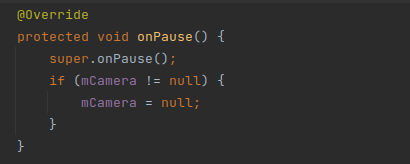
\includegraphics[width=0.8\textwidth]{Screenshot from 2023-02-22 19-51-26.png}
	\caption{Содержание метода onPause}
	\label{fig:activity:onPause:content}
\end{figure}

\subsubsection{Возобновление явления}
При возобновлении явления система вызывает метод onResume().\par
Важно помнить, что этот метод система вызывает каждый раз при
возвращении фокуса явлению, в том числе при первом запуске приложения.
Поэтому в методе onResume() нужно инициализировать те компоненты,
которые освободили в методе onPause(), и которые могли измениться за
время пока явление не было возобновлено.\par
Пример, показанный на рисунке \ref{fig:activity:onResume:content}, применения
onResume() сочетается с примером onPause(), который мы рассмотрели выше.
Здесь мы заново инициализируем камеру, которая была освобождена во время
паузы явления.
\begin{figure}[h!tp]
	\centering
	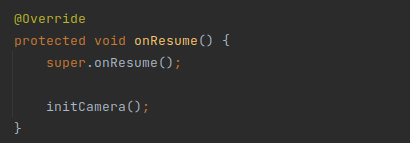
\includegraphics[width=0.8\textwidth]{Screenshot from 2023-02-22 19-52-34.png}
	\caption{Содержание метода onResume}
	\label{fig:activity:onResume:content}
\end{figure}

\section{Остановка и перезапуск явлений}
Остановка и перезапуск явлений, это важные процессы жизненного цикла,
которые гарантируют пользователю, что их данные не потеряются. Вот
небольшие примеры остановки и перезапуска явлений:

\subsection{Остановка явления}
Когда явление получает вызов onStop(), оно уже невидимо пользователю и
в этот момент нужно освободить все неиспользуемые ресурсы. Система может
уничтожить экземпляр остановленного явления, чтобы освободить память. В
критичных случаях система может убить процесс вашего приложения без
вызова onDestroy(), поэтому очень важно использовать onStop() для
освобождения ресурсов, пожирающих память.\par
Хотя перед вызовом onStop() вызывается метод onPause(), для выполнения
сложных операций, требующих интенсивной работы процессора (таких как
запись в базу данных), вы должны использовать onStop().\par
На рисунке \ref{fig:activity:onStop:content} показан пример метода onStop(),
который сохраняет переданную в активити сообщение.
\begin{figure}[h!tp]
	\centering
	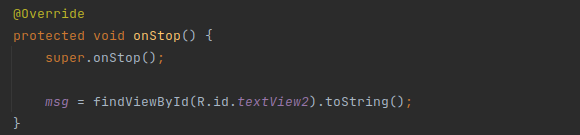
\includegraphics[width=0.8\textwidth]{Screenshot from 2023-02-22 20-10-08.png}
	\caption{Содержание метода onStop}
	\label{fig:activity:onStop:content}
\end{figure}

\subsection{Запуск и перезапуск явления}
Когда заново активируется явление после его остановки, вызывается метод
onRestart(). Система также вызывает метод onStart(), который срабатывает
каждый раз, когда приложение становится видимым(неважно было оно
запущено впервые или перезапущено). В то же время метод onRestart()
вызывается только когда приложение возвращается из остановленного
состояния. В нем можно выполнять действия, для явлений, которые были
остановлены, но не уничтожены.\par
Очень редко приходится использовать метод onRestart() для восстановления
состояния явлений, поэтому нет общепринятых правил по использованию
этого метода. Однако, поскольку onStop() полностью освобождает все
ресурсы явления, необходимо заново их инициализировать при
перезапуске. Но делается это так же при первоначальном запуске явления,
поэтому в подавляющем большинстве случаев приходится использовать для
этого метод onStart(), тем более, что он вызывается как при первоначальном
запуске приложения, так и при перезапуске.\par
Поскольку пользователь может надолго закрыть приложение, метод
onStart() подходит лучше всего для проверки существования всех
необходимых обектов (Рисунок~\ref{fig:activity:onStart:content}).
\begin{figure}[h!tp]
	\centering
	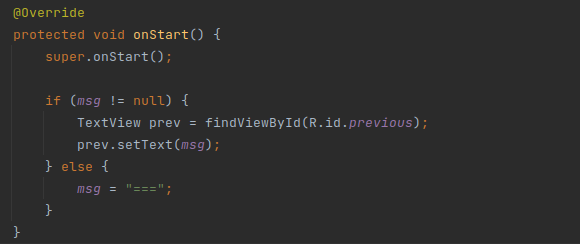
\includegraphics[width=0.8\textwidth]{Screenshot from 2023-02-22 20-20-55.png}
	\caption{Содержание метода onStart}
	\label{fig:activity:onStart:content}
\end{figure}


%====%
Обеспечить пересоздание явлений. Сохранить
состояния экземпляра явлений. Восстановить
состояния экземпляра явлений.
